\chapter{研究背景}\label{background}
本章主要介绍相关研究背景,首先说明智能体的基本概念;然后介绍当前热门的智能体架构-BDI(Belief-Desire-Intention)智能体架构;最后对BDI智能体在社会仿真场景下的相关现有研究进行细致阐述,其中包括对传统意图进展问题的研究,norm约束下BDI智能体决策问题的研究,对维持型目标的研究以及时序逻辑在BDI智能体中的应用。
\section{智能体系统}
智能体在现代社会有着广泛的应用,然而不同领域对智能体的定义也不尽相同。本文遵循\cite{DBLP:journals/ker/WooldridgeJ95}中对智能体的定义,智能体是一种处于一定环境下能够自主、智能地完成其他个体指派任务的计算机系统,其遵循感知--执行动作的周期性运作流程。其最大的特点是自主性、社会性、反应性以及主动性。
\begin{itemize}
  \item 自主性:自主性是智能体最核心的特性,其指的是指智能体能够自主地进行一系列行为,比如判断、计算和做出动作,以实现人们指定的目标。这种自主的表现都是基于内部状态和智能体的行为能力,内部状态是智能体对自身所处状态的理解,即智能体认为它是怎么样的、处于什么状态、目的是什么。而行为能力是指智能体根据内部状态进行自主的判断,能做出一些具体的行为来影响其周围的环境或改变自身的处境。自主性使得智能体决策以及行为由其自身控制,而非由其他个体操纵。
  \item 社会性:在多智能体系统(Multi-Agent Systems,MAS)中,智能体之间会进行交互,比如合作完成任务,或者在比赛中竞争,表现出社会性。在社会性的交互中,信息交流是不可或缺的,智能体须通过交流的语言、协议、信息本身对信息进行发送或接收处理,同时智能体根据交互的信息对系统中其它智能体建立认知模型,以更好地使智能体共同完成一些特定目标。
   \item 反应性:智能体能够感知到环境中的事件或发生的一些变化并及时的做出一些决策或行为来进行响应,以便实现指定目标。这种能力使得智能体在完成指定目标的过程中能够更加灵活地应对环境中的变化。
   \item 主动性:智能体的行为是以目标为导向的,其能够主动采取行动来实现给定的目标,而不是完全被动地等待,拒绝尝试对实现目标有帮助的行为。
\end{itemize}
% @TODO maybe consider other features?
\section{BDI智能体架构}
实现智能体的方式有多种,不同的实现方式对应了不同的智能体架构。目前已有多种智能体架构被提出,例如慎思型智能体架构(Deliberative agent Architecture),反应型智能体架构(Reactive Agent Architecture)以及混合型智能体架构(Hybird Agent Architecture)。本文的关注重点为BDI智能体架构(Belief-Desire-Intention Agent Architecture)。BDI智能体架构是当前热门且成熟的智能体架构,其起源于Bratman的关于实践推理(Practical Reasoning)的哲学理论\cite{bratman1987intention}。为了对人类的心理状态进行模拟,BDI智能体架构明确地将智能体的内部状态以一组特殊的数据结构表示,即信念、欲望和意图。基于BDI智能体架构的智能体被称为BDI智能体。
% Bielief
在BDI智能体中,信念表示的是BDI智能体所相信的事件或状态,例如在某个位置、目前的速度或当前的外部环境情况等等,然而信念并不一定是事实,仅仅代表BDI智能体的认知,BDI智能体会根据自身对环境的感知或自身做出的行为改变环境进而改变信念,或是将信念作为参考做出一系列的判断或行为。
% Desire
愿望指的是BDI智能体想要实现的环境环境状态。欲望可以是没有具体实现方案去实现的,甚至不可实现的,也可被视为一些未实例化的想法,而并没有确定去如何做,做什么。此外当智能体同时有多个意图时,由于没有实例化或决定实现这些意图,意图与意图之间可以有冲突,例如BDI智能体可以同时拥有进行休眠充电和打扫卫生这两个愿望,即使这二者是相互冲突的。
% 目标
目标(Goal)指的是一组智能体确定要去实现的愿望,也就是说一个目标对应于一个实例化的愿望,即智能体知道要实现什么并且承诺尝试去实现。目标的种类主要有两种:实现型目标(Achievement Goal)和维持型目标(Maintenance Goal)。
% acheivement goal
实现型目标表示智能体想要达到的世界状态,一旦该状态达成,其相应的实现型目标就会被丢弃。例如,智能体有一个去超市电池的实现型目标,一旦购买成功,无需重复购买,智能体便会丢弃该目标。

% Maintenance goal
维持型目标要求智能体在一段时间内(或者一直)维持某一世界状态。和实现型目标不同的是,维持型目标被满足后并不会被丢弃,而是仍然存储于智能体的内部。智能体会对维持型目标持续监控,直到其过期。在此期间一旦维持型目标被破坏,智能体便会尝试修复该目标状态,这种情况下智能体对待维持型目标的方式是被动的,即等到维持型目标被破坏再尝试修复,以被动方式应用的维持型目标被称为被动维持型目标(Reactive Maintenance Goal)。此外,智能体还可以在维持型目标被破坏之前对其是否在将来会被破坏进行预测评估,如果预计在将来的某个时刻维持型目标会被破坏,智能体还可以采取主动措施防止其被破坏,以该种主动方式应用的维持型目标被称为主动维持型目标(Proactive Maintenance Goal)。在本文中,维持型目标是一个重要的研究内容;后文将对维持型目标的相关调度算法进行细致阐述并进行性能评估。

%Intention
意图(Intention)为实例化的计划,用以实现某个目标。而计划的内部--计划体由动作和子目标组成。动作的执行可以直接影响外部环境,而子目标可由其他子计划实现。 当智能体承诺要实现某个目标时,便需要执行一个具体的计划来实现对应的目标。一个目标可由多个不同的计划来实现,智能体只要选择其中一个计划执行即可,即智能体会从该目标对应的可选计划中根据具体实际情况,判断并选择一个计划,通过执行选中的计划来完成相应目标,这种多个计划的设计也使得智能体可以灵活应对不同的环境。由于计划体也可以包含子目标,在运行过程中,会递归性地选出并执行多个计划,从具体实现的角度来说,每个意图都是一个栈,里面存储的就是部分实例化的计划,意图的执行也就对应于执行栈中一系列的计划。

% Practical Reasoning
在BDI智能体架构中,智能体进行决策的流程被称为实践推理(Practical Reasoning)。和纯粹的逻辑推理或理论推理不同,实践推理是以行为为导向的,即决定做什么以及如何去做。例如,假设Alice是Bob女儿,Carl是Alice的儿子。则基于逻辑推理可知Carl是Bob的孙子,该种推理方式仅仅依赖智能体的信念以及一些逻辑规则;相较于此,决定该乘坐何种交通工具上学的决策过程则是实践推理的范畴,因为其包含对“如何做”的考虑,是以行为为导向的推理。

% deliberation and means-ends reasoning
Bratman\cite{bratman1987intention}认为实践推理可被看做智能体基于其内部状态,(即信念、愿望等),在多个相互冲突的选择中进行权衡考量,做出合理的决策的过程。
%
具体地,实践推理主要有两步构成:慎思(Deliberation)和手段推理(Means-Ends Reasoning)。
%
在第一步慎思过程中,智能体考虑要去实现哪个目标,即生成目标对应的意图,意味着智能体决定要去尝试实现该目标。
%
而在第二步手段推理过程中,智能体考虑如何实现某个目标,即对于上一步确定要实现的目标,决定执行哪一个计划去实现。
% example
例如,假设智能体现有两个愿望:前往超市购买食物和在家打扫卫生;在经历慎思过程后,智能体决定前往超市。而前往超市有两种途径:走路前往和开车前往;智能体决定走路前往还是开车前往的过程即为手段推理。

\subsection{BDI智能体程序的执行}
为了实现BDI智能体程序,Bordini\cite{bordini2007programming}描述了BDI智能体运行的控制流,其具体流程如图\ref{fig:deliberation}。
\begin{figure*}[htb]
\centering
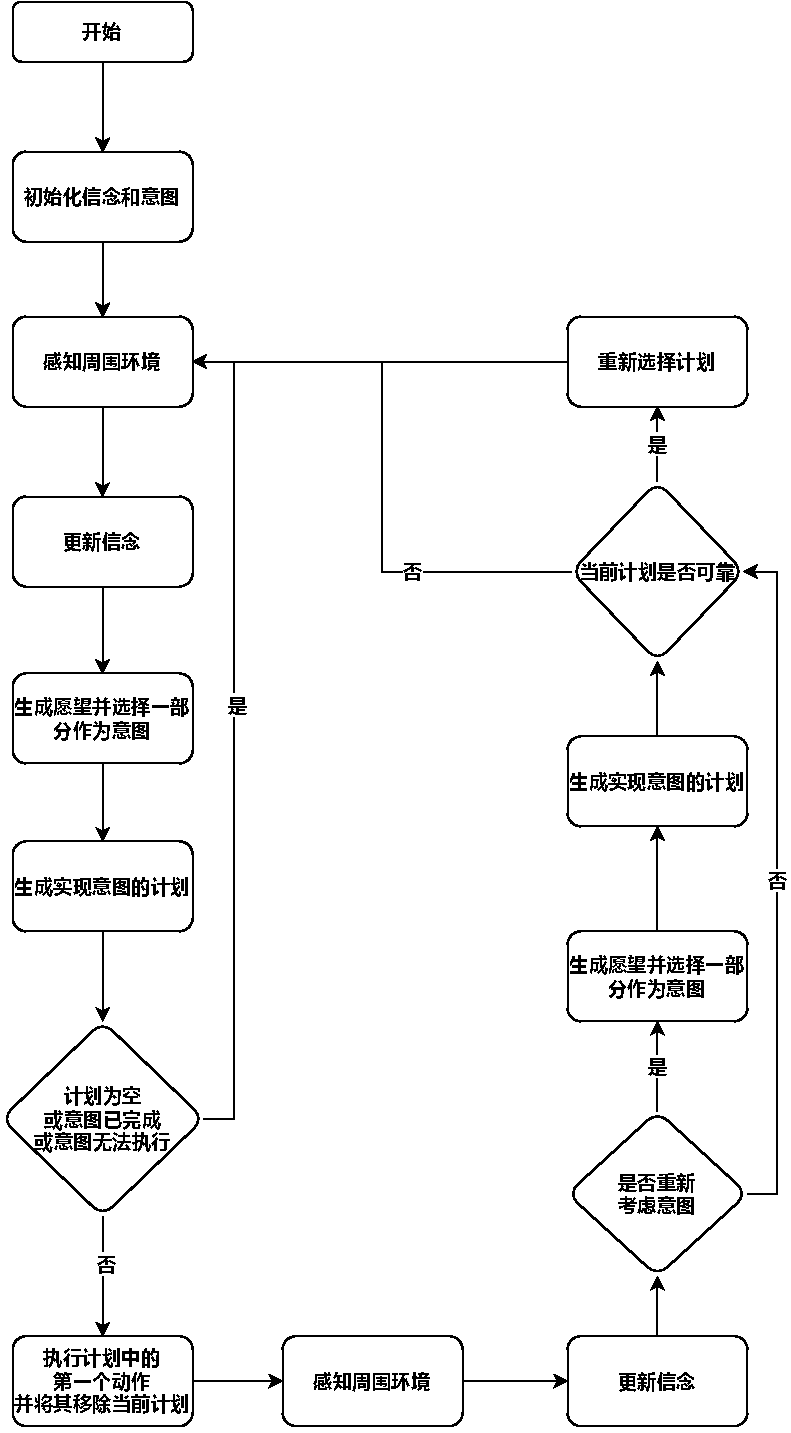
\includegraphics[scale=0.6]{./figs/deliberation_cycle}
\bicaption{BDI智能体的执行流程}{Overall control loop of BDI agent}
\label{fig:deliberation}
\end{figure*}

在执行动作之前,智能体首先对周围环境进行感知,并对自身的信念进行更新,然后智能体根据更新后的信念以及当前的意图得到新的愿望,并选择部分愿望生成对应的意图,最后选择计划以实现意图。理想情况下,在具体执行时智能体依次执行计划中的每一个动作直至计划计划中的所有动作都执行成功。然而,由于环境是多变而不确定的,智能体在执行完一个动作之后需要对环境进行感知并更新其信念,并决定是否要重新考虑意图。由于重新考虑意图需要额外的计算开销,通常情况下智能体不会频繁地进行重新考虑的操作,而是当确定重新考虑会对当前的意图造成改变时进行该操作。即如果重新考虑不会对当前意图造成影响,那么智能体无须在执行过程中浪费计算资源而是直接执行当前的意图。最后,无论是否重新考虑意图,智能体判断当前的计划是否依然合理或是否值得继续执行。如果当前计划被判断为不适合继续执行,智能体将重新进行计划选择。

\section{国内外研究现状}
本节对现有相关研究进行文献述评,分别考虑了对经典意图进展问题的相关研究,对维持型目标的相关研究以及norm约束下决策问题的相关研究。
% 考虑分三点:1.传统意图进展问题,2.norm约束下的决策,3.维持型目标下的决策
\subsection{经典意图进展问题研究现状}
% SI
在对意图进展问题的研究中,Thangarajah等人\cite{DBLP:journals/jar/ThangarajahP11,DBLP:conf/ijcai/ThangarajahPW03}提出了基于SI (Summary Information)的意图调度算法,其通过自底向上总结信息的方式确定实现目标的必要条件、可能条件、必要结果以及可能结果来推理出意图之间是否存在冲突以及是否存在协同效应。SI算法在智能体程序编译期进行信息总结计算,并在运行期间随着智能体意图的进展动态更新总结信息。此外,SI支持实时判断接收新目标的机制,允许智能体在运行时根据总结信息判断新的目标是否一定会、可能会或一定不会与当前目标相冲突,然后决定是否接收新的目标。然而,该方法假设现有目标的优先级总是大于新目标,若发生冲突则不接收新目标,而不会考虑抛弃现有的冲突目标。

% C
Waters等人\cite{DBLP:conf/atal/WatersPS14,DBLP:conf/aamas/ThangarajahSP12}提出了CB(Coverage Based)意图调度算法,并在后续研究中对其进行了改进\cite{DBLP:journals/aamas/WatersPS15}。CB考虑在编译期对实 现目标计划的健壮性进行数值化刻画,提出在不同环境下智能体实 现某个目标的可执行性(Coverage),以及在同一环境下智能体实现 某个目标的计划选择多样性(Overlap)。在意图进展过程中CB优先考虑实现脆弱的目标,以免因为环境自身的动态性导致目标因无可选计划执行而无法实现。相较于SI,CB重点考虑的是智能体在动态环境下的意图进展。

% MCTS
Yao等人提出了基于蒙特卡洛树搜索(Monte Carlo Tree Search,MCTS)的意图调度算法\cite{DBLP:conf/aaai/YaoLT16,DBLP:conf/atal/YaoL16,DBLP:conf/ecai/YaoLT14,DBLP:conf/atal/Yao21,DBLP:conf/ijcai/Yao20,DBLP:conf/ecai/YaoLT16},其利用MCTS的特点,专注于对最有前景的行为进行搜索,并基于随机模拟构建并不断扩展搜索树,最终根据用户自定义的评判标准和搜索树记录信息得到决策结果。和SI以及CB不同,MCTS算法的执行发生在程序运行期,其总是基于当前状态对决策空间进行搜索,并得出当前决策结果。MCTS调度策略被应用于消 解并行意图间的冲突、开发并行意图交错执行的协同效应、对时间 限制的意图进行调度以及在动态和不确定环境下的意图调度。此外,根据对目前该研究领域的调研,得知基于MCTS的意图调度算法 是当前可验证的最好的意图调度策略。
% 传统意图调度方法的问题
然而,上述方法都没有考虑到社会模拟场景中维持型目标对智能体的影响,缺乏在意图调度是考虑维持型目标的能力。


\subsection{维持型目标研究现状}
% maintanance goal
在对维持型目标的研究中,Duff等人提出一种基于SI的意图调度算法\cite{DBLP:conf/atal/DuffHT06},其在决策过程中加入对维持型目标的考虑:若实现型目标将与维持型目标冲突,执行预防措施(例如补充资源)。 然而,和SI类似,该算法假设当前的目标优先级总是高于新的目标,并且如果新的目标为维持型目标且与当前目标相冲突,维持型目标将被直接抛弃。后来Duff等人在\cite{DBLP:journals/ci/DuffTH14}中拓展了维持型目标的规范语法及语义,但是意图调度策略并没有被改进。Hindriks等人\cite{DBLP:conf/dalt/HindriksR07}提出了一种处理维持型目标的决策机制,该机制直接避免执行破坏维持型目标的行动,保证维持型目标不会被破坏。然而该方法将会导致智能体可执行的行动变少,降低智能体的灵活性。Thangarajah等人\cite{DBLP:conf/ecai/ThangarajahHMY14}分析了维持型目标的进展过程, 提供了一套合理的维持型目标进展模型,但是起没有考虑到意图进展问题。

目前在BDI智能体研究领域中,已有多种对智能体的功能性进行拓展的方法被提出以提升其适用性。鉴于大多数对智能体目标的研究 都着重关注实现型目标和维持型目标,Dastani等人\cite{DBLP:conf/atal/DastaniRW11}提出以时序逻辑来表示目标,以拓展智能体支持的目标种类。在他们提出的框架中,目标的表示不仅包含基本命题,还包含时序连接符号如$\diamond$(最终),$\square$(总是)以及$U$(直到)。在具体应用时,由于大多数智能体语言和平台都不支持时序逻辑,需要将时序逻辑表示的目标转化为一般化的实现型目标和维持型目标以便用于实际使用。Dastani等人提出操作化(Operationalization)方式,根据时序连接符不同,对时序逻辑表示的目标进行合理转化,使其转变为一个或多个逻辑对应的实现型目标和维持型目标。然而,该框架并没有提供一个一般性的意图调度算法,某些特殊形式的目标仍然需要用户自定义条件-动作对,虽然有一点的拓展性,但加重了用户的负担;此外,该框架也没有考虑到社会仿真场景下的norm,这导致其不适用于norm约束场景。
\subsection{Norm约束下的决策问题研究现状}
% norm决策
% BOID
在norm对智能体决策影响的研究领域中,最早或许可以追溯到BOID架构\cite{DBLP:conf/agents/BroersenDHHT01},BOID架构实质上是对BDI架构的一种延申,赋予其决策时考虑norm的能力。BOID在BDI的基础上引入了智能体性格类型的概念以处理norm与行动、目标之间的冲突。BOID智能体可以是社会型的、无视规范型的等,不同类型的BOID智能体对norm有不同的解释,在解决norm相关冲突时也有不同的策略。例如无视规范型的智能体会更倾向于考虑自身目标的实现,而不过多考虑norm对其约束,在norm相关冲突发生时忽略norm的存在。BOID智能体的决策过程是纯粹基于命题规则的。如果在其决策过程中某些规则发生冲突(可能由norm造成),智能体将基于其自身类型进行冲突消解以得到最早确定的决策结果。BOID架构的设计非常简洁,易于理解,但是这种架构并没有广泛的实际应用。很大 一部分原因在于其健壮性低下,仅依靠逻辑推理做出决策,决策过程的时间复杂度高,当规则量庞大时,极其耗时,且不易维护。

% NoA
NoA\cite{DBLP:conf/ijcai/KollingbaumN03}架构基于BDI架构并引入了norm的相关概念,例如义务,禁令以及许可。许可规范了智能体可以做什么(而不一定要去做)。在决策阶段,NoA架构规范了智能体该从计划库中选择哪个计划去执行以遵守norm的相关约束。NoA是完全以norm为主导的架构,它没有自身内部的目标,因此不需要考虑norm与目标的冲突。这使得NoA总是会做出遵守norm的行动。NoA能够处理norm的相关概念,其架构设计也较为简易,易于理解。然而--中仅使用文字对NoA的概括性描述,而缺乏对NoA架构抽象准确的形式化定义。没有内部状态,完全以norm为导向的设计也使得NoA架构适用场景受限,限制了BDI智能体的基本自主性。


基于norm的行为修改(Norm-based Behavior Modification,NBM)\cite{DBLP:conf/atal/MeneguzziL09}是对基础BDI架构的一种延伸,其解决的问题主要是智能体在运行时如何去适应新的norm,NBM架构的重点在于提供一种机制使得智能体有能力在运行时去约束一些计划的执行以适应其在运行时所检测到的新的norm。其优点在于其方法依然在BDI的框架下,对于新的norm,创建一个新的计划来处理,将那些norm禁止的计划进行限制,不让其在后续norm生效的情况下执行。该机制可以方便地部署到其它符合BDI架构的智能体系统中。虽然本文实现了在运行时应对新检测的norm的机制,但是没有对norm对于智能体的影响进行精确地刻画,简单认为norm禁止的计划就不能去执行,使得智能体灵活性降低。其研究重点关注的问题也仅限于计划选择,目标选择并不在其考虑范围之内。

% N-2APL
N-2APL\cite{DBLP:conf/aamas/AlechinaDL12}是基于2APL\cite{DBLP:journals/aamas/Dastani08}的智能体编程语言。 N-2APL在2APL的基础上拓展了对norm的表示与处理机制,支持表示义务、禁令等概念,支持在决策过程中处理norm带来的冲突。N-2APL的目标选择与计划选择机制是基于实现目标截止期限以及计划优先级制定的。N-2APL假设计划优先级由编程人员根据norm的影响提前定义。其决策过程主要为: 1.放弃某些低优先级的目标以确保高优先级的目标能够在截至期限内完成;2.选取一个高优先级且能够在截止期限实现的目标;3.根据提前定义好的优先级顺序选择计划执行。
在N-2APL中,有限制条件的义务并没有被考虑,使其应用场景受限。N-2APL通过引入原子计划与非原子计划的概念,以降低可能的执行序列的数量来控制决策算法的时间复杂度并消解计划间并行执行的冲突:原子计划执行时不能被打断,而非原子计划执行过程中可以被其他计划打断。这种设计需要编程人员手动对计划进行分类,不利于大规模实践应用;由于可能执行序列的减少,这种设计也会一定程度上降低了BDI智能体的灵活性。

% N-Jason
N-Jason\cite{DBLP:conf/dalt/LeePLDA14}是一个基于Jason\cite{bordini2007programming}智能体编程语言,支持运行时处理未知norm智能体编程语言。相较于以往的norm处理机制——假设norm在运行前就已经确定,在运行时也不会改变, N-Jason支持运行时对未知norm的识别。如果N-Jason识别到义务norm,则将其转化为一个新的目标待后续阶段实现;如果识别到禁令norm,则将其加入禁令norm集合,供后续进行冲突消解阶段应用。与N-2APL类似,N-Jason 也支持基于截止期限与norm的影响对目标、 计划划分优先级以消解冲突并选择合适的计划执行。然而,不像N-2APL,N-Jason没有考虑多目标之间的选择问题,仅考虑了如何选择计划。作者也提到基于N-Jason产生的的智能体行为可能在编程人员看起来是不可解释、不可预测的,然而却没有提供确切的理论或实践依据。

% v-BDI
v-BDI\cite{DBLP:journals/eaai/MeneguzziROVL15}对BDI架构进行了拓展,在决策时加入了对norm的考虑,其允许智能体在norm冲突发生时,根据自身认识自主地选择是否遵守norm,v-BDI的关键技术在于在计划选择时先对各计划的行动进行模拟运行,然后根据模拟结果对比各个计划的价值,最终选择出价值最大的计划执行。v-BDI依据计划价值来进行计划选择, 当执行计划的收益大于违反norm受到的惩罚时,智能体可以选择去做出违反norm的行为以获得更大的整体收益。这种机制保留了BDI智能体的灵活性与自主性,同时计划选择的标准由模拟结果决定, 不需要编程人员明确给的。编程人员仅需要定义模拟的价值函数即可。v-BDI中对计划价值的计算仅考虑其中的行动,而不考虑子目标,这使得价值计算过程的时间复杂度较低,易于实际的应用。然而v-BDI仅考虑到了计划选择问题,而并没有提及多目标情况下的目标选择问题。仅考虑计划中行动的模拟机制虽然高效,但是必然会因为没有考虑到子目标而导致价值计算不准确。

此外,在非BDI架构领域,也有一些对norm考虑的决策机制被提出。相较于BDI架构,非BDI架构的智能体没有事先由编程人员定义好的计划库,而仅有由一个个独立的行动组成的行动集合。因此,设计非BDI架构智能体norm决策机制最大的挑战在于如何在norm规范下根据一定的规则,基于行动集合生成某些执行序列以供智能体执行,达到设计者的设计目标。

%
Shams等人\cite{DBLP:conf/atal/ShamsVPV15}提出的方法使用到了提前设定好的计划,但是其和BDI智能体的差异在于Shams等人提出的决策过程允许智能体根据norm的影响动态调整执行计划。其在运行时选择执行序列并将其与当前计划相比较,若新执行序列组成的计划的收益大于当前计划,则将新生成计划作为当前计划执行。Norm对智能体行为的约束体现在若智能体做出违反norm的行为将受到一定数值的惩罚。各行动受惩罚值的大小决定了智能体会如何执行计划:智能体总是会执行整体收益(实现目标的收益+违反norm的惩罚)最大的计划。该方法能够通过搜索得到最优的计 划,但是其时间复杂度较高,若可选计划数量较多,则实际应用较为困难;同时其也没有考虑到多个并行执行的计划之间的相互冲突与影响。

% RL
Li等人\cite{DBLP:conf/atal/LiMFL15}提出了使用强化学习方法对变化的或位置的norm进行学习,并根据学习结果对智能体自身的行为进行动态调整,以更好地在norm存在的环境中实现目标。Li等人\cite{DBLP:conf/atal/LiMFL15}分别对两种强化学习方法 Q-Learning 和 SARSA\cite{Sutton2005ReinforcementLA}进行了测试,验证了其有效性并对比分析了 两种方法的特点与适用场景:Q-Learning更加激进,对norm的学习的速度很快,但是不太稳定;SARSA比较保守,对 norm的学习速度慢,但是稳定性高。与—类似,\cite{DBLP:conf/atal/LiMFL15}没有考虑多目标之间的冲突问题,并且当问题规模较大时,这两种基础强化学习方法需要消耗大量计算时间,不利于实际应用。

% argumentation based
Shams等人\cite{DBLP:conf/ijcai/ShamsVOP16,DBLP:journals/taas/ShamsVOP20,DBLP:conf/atal/ShamsVPV15}提出的方法在不同场景设定下对 norm 的考虑主要体 现在可解释性,其实用 Argumentation Dialog 的方法试图对智能体 在 norm 约束下的行为进行解释,以提高人类对智能体程序的信任 度。同时,其考虑到了 norm 与智能体目标之间的冲突问题,提供了 一套消解冲突的机制。然而,与\cite{DBLP:conf/atal/LiMFL15}类似,在各个场景下该机制的 时间复杂度较高,并且没有考虑多个目标之间的冲突。


综上,目前对智能体在维持型目标的支持、norm约束下的决策以及对智能体目标种类的拓展方面的研究都取得了重要的进展。然而现有研究依然存在一些问题与空白。

现有的BDI模型不支持维持型目标,且目前对维持型目标研究也仅仅考虑单个目标的执行对维持型目标的影响,而没有考虑多目标并行执行的情况,因此无法有效解决引入维持型目标带来的问题。

现有的BDI慎思过程框架缺乏对norm的支持,使得智能体在决策时无法考虑到norm对其行为的约束作用,进而无法做出合理的决策;同时,现有的对BDI智能体意图调度的相关研究也并没有考虑到norm对智能体的影响,使得其无法用于解决norm约束下智能体意图调度问题。

现有的相关研究大多仅针对社会仿真场景下的某一方面的问题(例如仅针对norm或维持型目标),而没有考虑norm和维持型目标共存的情况,缺乏一般性。
